\question Consider the bipartite graph below. Let the matching
\(M=\{A h, C i, D j, E k\}\). Apply augmenting path algorithm to
extend the size of this matching. Clearly explain your step.

\begin{center}
  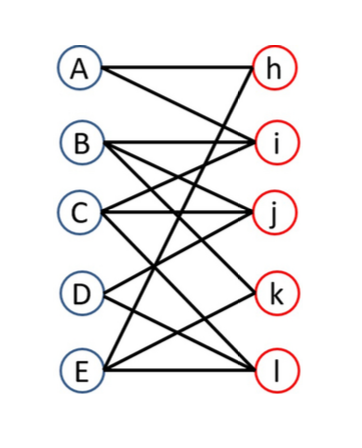
\includegraphics[width=0.35\textwidth]{figures/p2-graph}
\end{center}

\begin{solution}
  We first start at the unmatched vertex \(B\). Then, we visit
  \(j\), \(D\), and \(l\) in that order. Since we've arrived at
  the unmatched vertex \(l\), we will backtrack and augment our
  original alternating path:
  \[
    B \underset{\text{unmatched}}{-} j \underset{\text{matched}}
    {-} D \underset{\text{unmatched}}{-} l
  \]
  Namely, we add edge \(Dl\) and remove edge \(Dj\).
  We also add edge \(Bj\). We now end up with augmented path
  \[
    B \underset{\text{matched}}{-} j \underset{\text{unmatched}}
    {-} D \underset{\text{matched}}{-} l
  \]
  Since this is already a perfect matching, we cannot extend it
  anymore. Hence, we have a new matching 
  \[
    \{Ah, Bj, Ci, Dl, Ek\}
  \]
  Below is (left to right): initial, alternating path (blue),
  final states of the graph. It may be a bit hard to see, though
  :P

  \begin{center}
    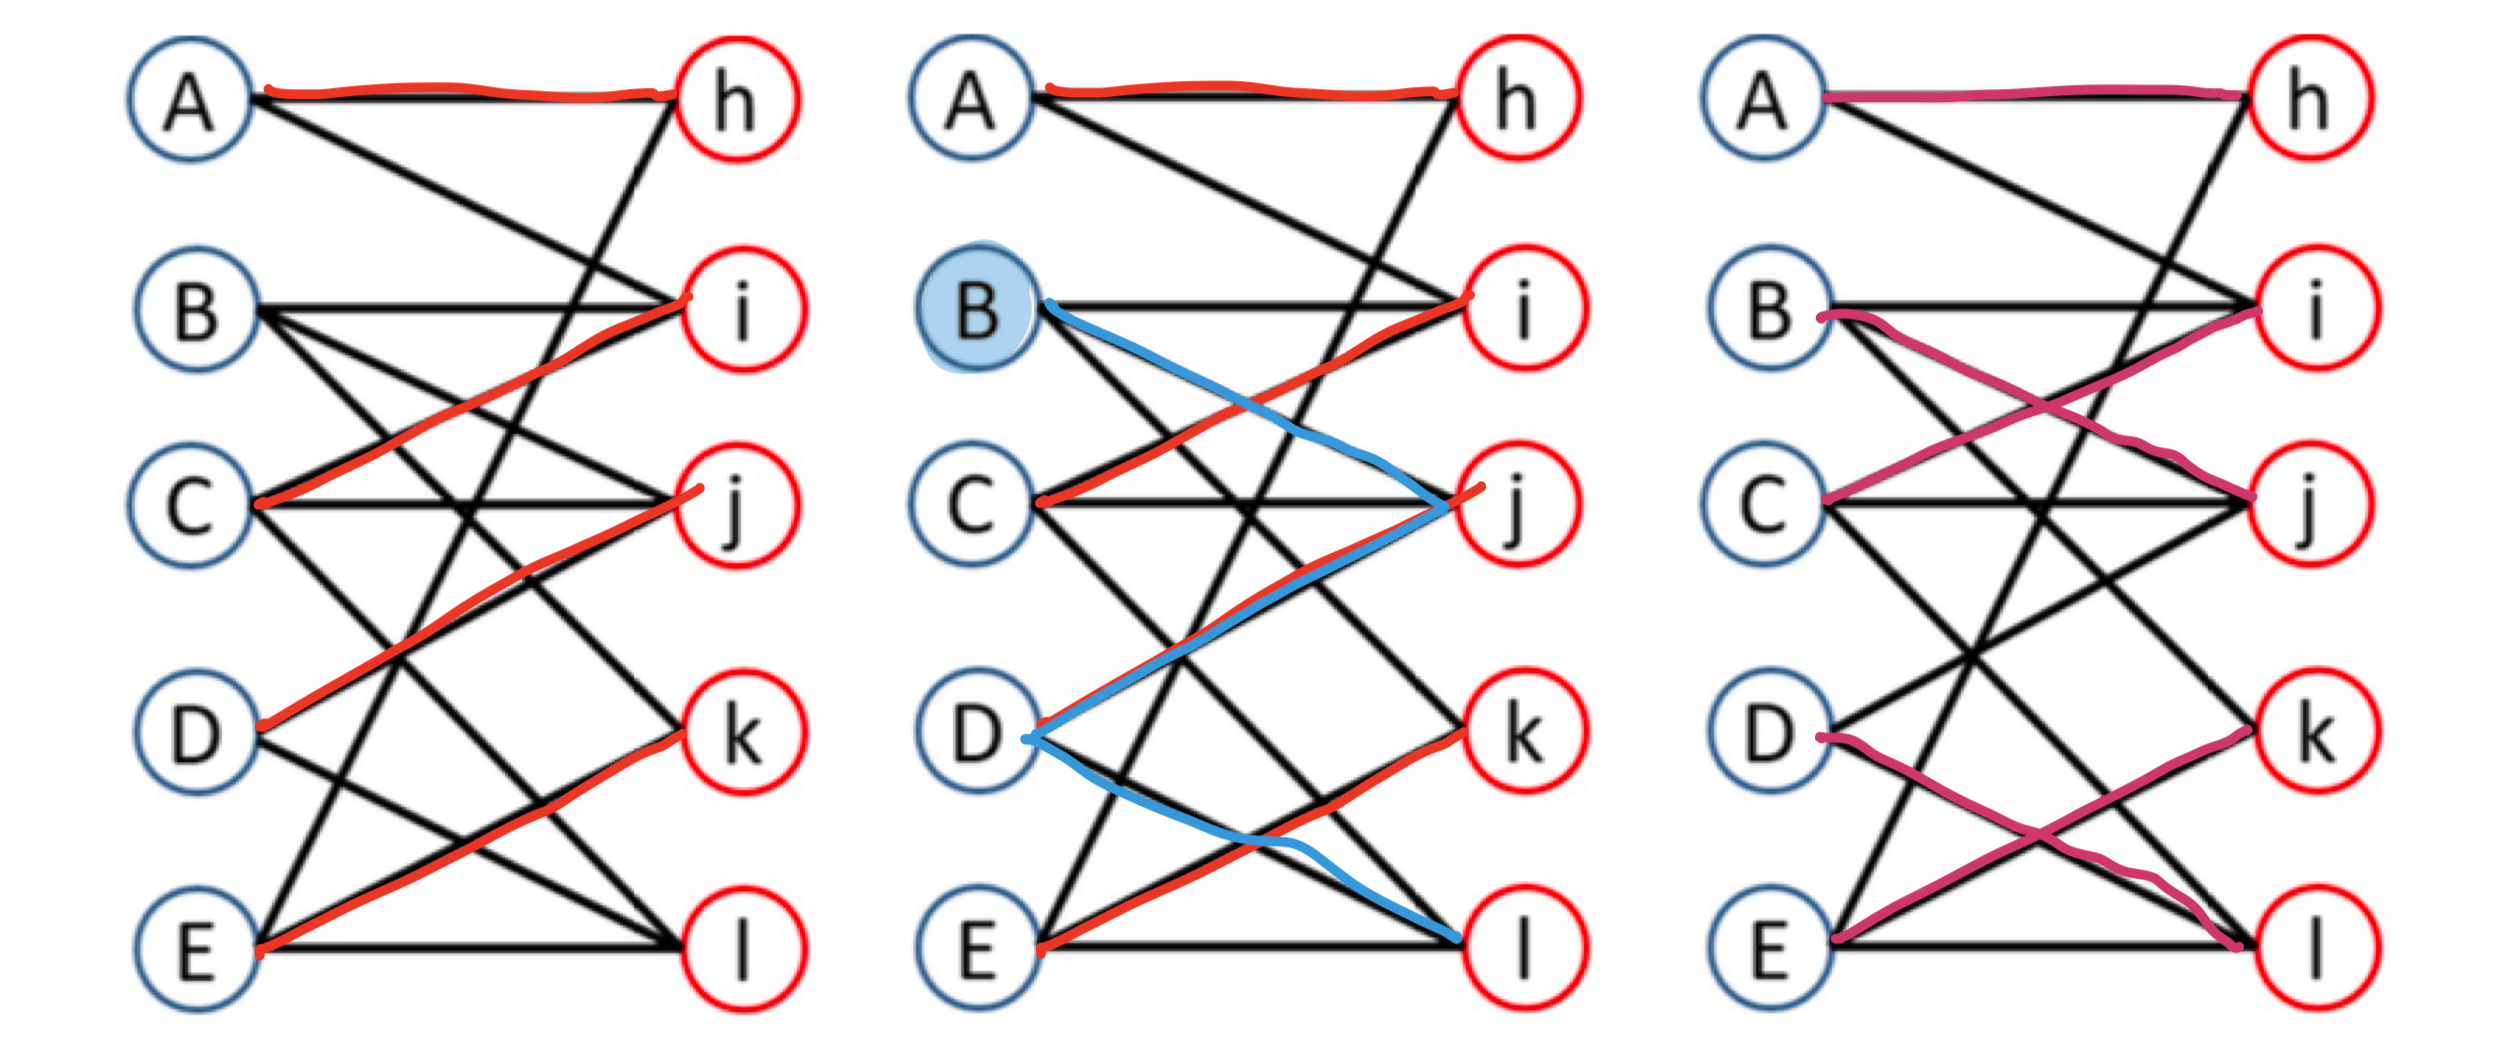
\includegraphics[width=0.69\textwidth]{figures/p2-soln}
  \end{center}
\end{solution}
